\section{Conclusion}
This applicative project and first part of the sigma racing was very interesting. \\
We learned a lot and we now know that we are really pasionate about image recognition and deep learning.\\

It is a very complex domain and we are far from mastering it. Nevertheless, we have done our best in order to make a working model. We took deep learning online classes and read books to complete our train. It seemed, at first, very complexe (mostly the mathematicals aspects, and its still is !) but we managed to understand the basics and we are learning more every days.\\

This project will come to an end on June 2021. The next step is to buy the car and implement all the work that we have done inside it. We also plan to design our own removable track with the same specifications as the official one in order to test the car in different track configurations. Moreover, we will need to get cracking on the obstacles detections (is a Lidar sensor usefull ?) as well as the start and finish behaviors of the car.\\

We are still struggling with the hardware as we cannot borrow a GPU for the schools servers. It has a direct affect on the duration of the training and some help in this area would be more than welcome.

\hfill \\ 

\begin{figure}[!h]
\centering
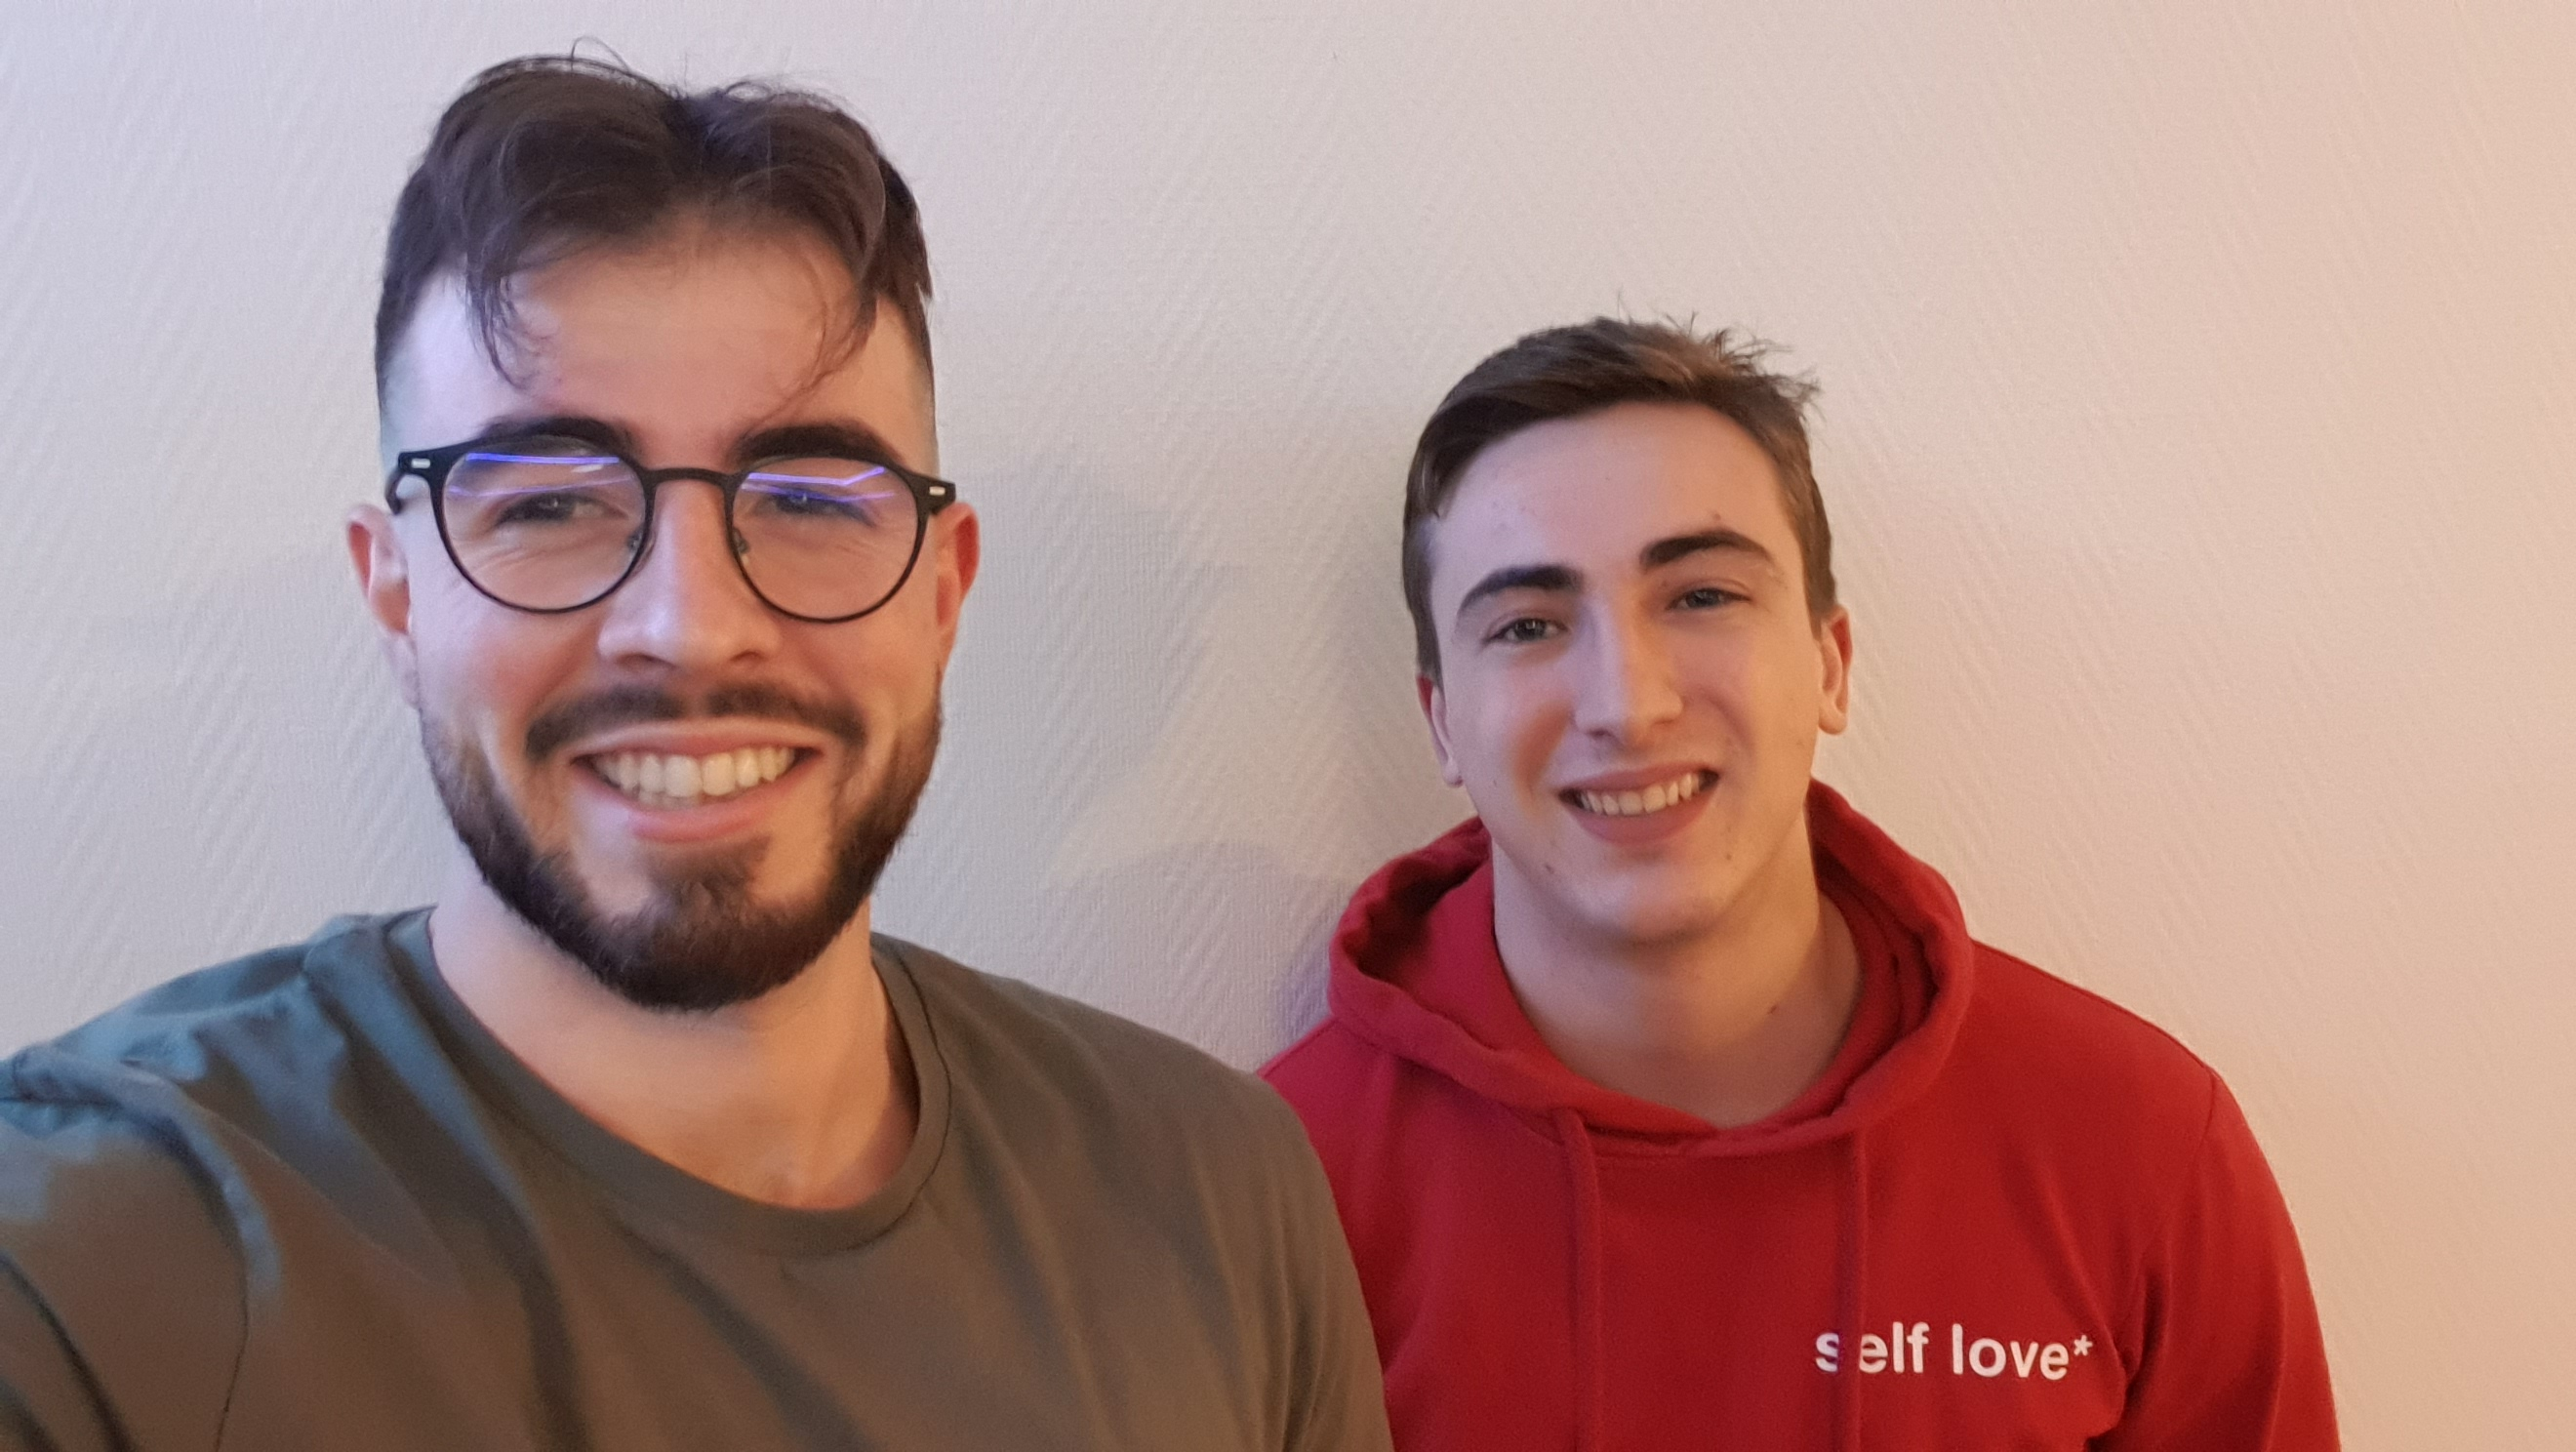
\includegraphics[scale=0.15]{img/girou_barbault.jpg}
\caption{Romain (left) and Cyprien (right)}
\end{figure}
\clearpage